\documentclass{G7-32}
\usepackage{xurl}
\sloppy

% Поля по нормоконтролю (верх/низ 20 мм, слева 30 мм, справа 15 мм); класс G7-32 уже подключает geometry — уточняем параметры
\geometry{a4paper,top=20mm,bottom=20mm,left=30mm,right=15mm}

% Абзацный отступ 1,25 см, без дополнительного интервала между абзацами одного стиля (методичка п. 2.2.10)
\setlength{\parindent}{1.25cm}
\setlength{\parskip}{0pt}

% Запрет висячих строк (нормоконтроль п. 35)
\widowpenalty=10000
\clubpenalty=10000

% Настройки стиля ГОСТ 7-32
% Для начала определяем, хотим мы или нет, чтобы рисунки и таблицы нумеровались в пределах раздела, или нам нужна сквозная нумерация.
% \EqInChapter % формулы будут нумероваться в пределах раздела
% \TableInChapter % таблицы будут нумероваться в пределах раздела
% \PicInChapter % рисунки будут нумероваться в пределах раздела

% Добавляем гипертекстовое оглавление в PDF
\usepackage[
bookmarks=true, colorlinks=true, unicode=true,
urlcolor=black,linkcolor=black, anchorcolor=black,
citecolor=black, menucolor=black, filecolor=black,
]{hyperref}

\urlstyle{same}

\usepackage{pdfpages}
\usepackage{pdflscape}

% Изменение начертания шрифта --- после чего выглядит таймсоподобно.
% apt-get install scalable-cyrfonts-tex

% \IfFileExists{cyrtimes.sty}
%     {
        % \usepackage{cyrtimespatched}
%     }
%     {
%         % А если Times нету, то будет CM...
%     }

\usepackage{graphicx}   % Пакет для включения рисунков
\usepackage{grffile}    % поддержка имён файлов с пробелами
\graphicspath{{images/}}

% С такими оно полями оно работает по-умолчанию:
% \RequirePackage[left=20mm,right=10mm,top=20mm,bottom=20mm,headsep=0pt]{geometry}
% Если вас тошнит от поля в 10мм --- увеличивайте до 20-ти, ну и про переплёт не забывайте:

% Пакет Tikz
\usepackage{tikz}
\usetikzlibrary{arrows,positioning,shadows}

% Произвольная нумерация списков.
\usepackage{enumerate}

% ячейки в несколько строчек
\usepackage{multirow}

% itemize внутри tabular
\usepackage{paralist,array}

% Таблицы
\usepackage{amsmath} % equation, \eqref
\usepackage{array} % расширенные возможности для работы с таблицами
\usepackage{tabularx} % автоматический подбор ширины столбцов
\usepackage{dcolumn} % выравнивание чисел по разделителю

\usepackage{setspace} % полуторный интервал (нормоконтроль п. 25)
\setstretch{1.5}

\newenvironment{compactlist}{%
    \renewcommand{\labelenumi}{\hspace{6.5mm}\arabic{enumi})}
    \setlength{\topsep}{0pt}%
    \setlength{\partopsep}{0pt}%
    \setlength{\itemsep}{0pt}%
    \setlength{\parsep}{0pt}%
    \begin{enumerate}%
}{%
    \end{enumerate}%
}



\makeatletter
\renewcommand\theenumi{\arabic{enumi}}
\renewcommand\labelenumi{\hspace{6.5mm}\theenumi)}
\renewcommand\theenumii{\arabic{enumii}}
\renewcommand\labelenumii{\hspace{6.5mm}\theenumii)}
\renewcommand\p@enumii{\theenumi.}
\makeatother

\makeatletter
\renewcommand*\l@section{\@dottedtocline{1}{0em}{2.3em}}
\renewcommand*\l@subsection{\@dottedtocline{2}{0em}{3.2em}}
\renewcommand*\l@subsubsection{\@dottedtocline{3}{0em}{4.1em}}
\makeatother


\usepackage{caption}
\usepackage{ragged2e}

\DeclareCaptionJustification{centerednohyphen}{\Centering\hyphenpenalty=10000\exhyphenpenalty=10000}
\DeclareCaptionLabelSeparator{shortdash}{ \textendash\ }

\usepackage{float}
\setlength{\floatsep}{0pt}
\setlength{\textfloatsep}{0pt}
\setlength{\intextsep}{7pt}

\captionsetup{aboveskip=7pt,belowskip=0pt,justification=centerednohyphen,singlelinecheck=false,labelsep=shortdash}
\captionsetup[table]{justification=RaggedRight,singlelinecheck=false}
\captionsetup[figure]{justification=centerednohyphen,singlelinecheck=false}

\usepackage{chngcntr}

\usepackage{mdframed}
\usepackage{xcolor}

\mdfsetup{
linecolor=black,
linewidth=1pt,
roundcorner=5pt,
innerleftmargin=5pt,
innerrightmargin=5pt,
innertopmargin=5pt,
innerbottommargin=5pt,
skipabove=0pt, % Reduces space above the frame
skipbelow=0pt, % Reduces space below the frame
leftmargin=0pt, % Reduces left outer margin
rightmargin=0pt % Reduces right outer margin
}

% Листинги кода: listings (не minted — не требует pygmentize в PATH при сборке MiKTeX)
\usepackage{listings}
\renewcommand{\lstlistingname}{Листинг}
\lstset{
  basicstyle=\ttfamily\footnotesize,
  breaklines=true,
  columns=fullflexible,
  numbers=left,
  numberstyle=\tiny\color{gray},
  numbersep=8pt,
  stepnumber=1,
  frame=single,
  framerule=0.4pt,
  xleftmargin=2em,
  framexleftmargin=1.2em,
  tabsize=2,
  showstringspaces=false,
  extendedchars=true,
  keepspaces=true
}

\makeatletter
\let\oldtableofcontents\tableofcontents
\renewcommand{\tableofcontents}{%
  \begingroup
  \hyphenpenalty=10000
  \exhyphenpenalty=10000
  \oldtableofcontents
  \endgroup
}
\makeatother

\makeatletter
\def\@hangfrom#1{\setbox\@tempboxa\hbox{{#1}}%
      \hangindent 0pt%\wd\@tempboxa
      \noindent\box\@tempboxa}
\makeatother

\usepackage{etoolbox}
\AtEndEnvironment{lstlisting}{\vspace{-6pt}}
\AtEndEnvironment{table}{\vspace{-10pt}}
\AtEndEnvironment{center}{\vspace{-14pt}}
\AtEndEnvironment{figure}{\vspace{-14pt}}


\usepackage{fontspec}

% Указываем шрифты для основного текста и для кириллицы:
\setmainfont{Times New Roman} % если установлен в системе
\newfontfamily\cyrillicfont{Times New Roman} % для кириллического текста

% Убирает точку после номера главы
\makeatletter
\renewcommand{\thesection}{\thechapter.\arabic{section}}
\renewcommand{\thesubsection}{\thesection.\arabic{subsection}}
\renewcommand{\@seccntformat}[1]{%
  {\fontsize{14pt}{21pt}\selectfont\bfseries \csname the#1\endcsname}\hspace{1em}%
}
\makeatother

\usetikzlibrary{arrows.meta,positioning,shadows,shapes.geometric,calc}
\usetikzlibrary{shapes.multipart}

\hyphenpenalty=10000
\exhyphenpenalty=10000

\begin{document}

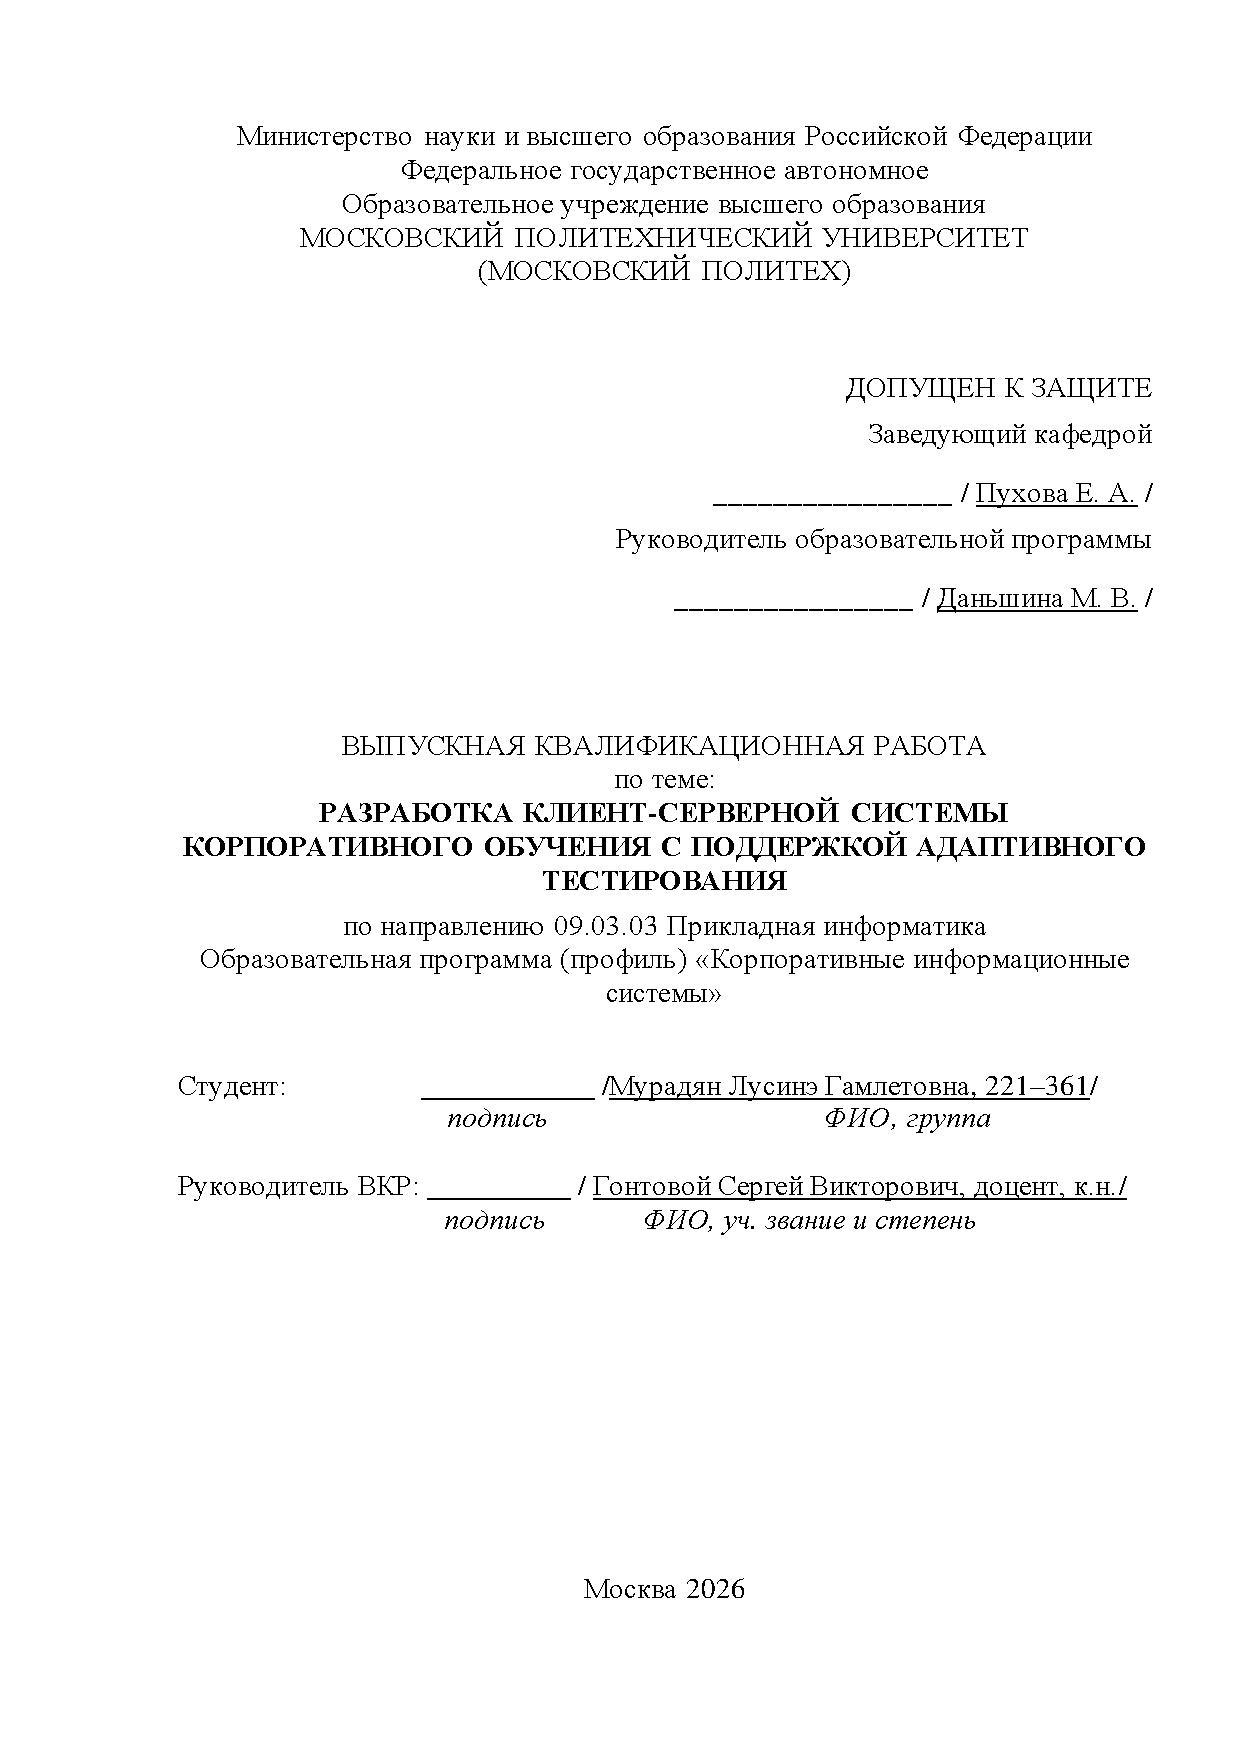
\includepdf[pages=1]{./extra/Title.pdf}
\newpage

\tableofcontents
\newpage

% Переопределение нумерации ONLY для этого документа
\makeatletter
\renewcommand{\thesection}{\arabic{section}}
\renewcommand{\@seccntformat}[1]{\csname the#1\endcsname\quad}
\makeatother

\setcounter{section}{0}

\section{Предметная область и актуальность}

Системы управления обучением (Learning Management System, LMS) используются в университетах и компаниях для организации онлайн‑курсов, тестирования и учёта прогресса обучающихся \cite{moodle,openlms}. Они обеспечивают хранение учебных материалов, проведение тестов, выставление оценок и формирование отчётов для преподавателей и руководителей.

Во многих распространённых LMS основное внимание уделяется веб‑доступу и линейным учебным курсам, одинаковым для всех пользователей \cite{moodlecloud}. В условиях роста доли мобильного обучения и сокращения времени, которое сотрудники и студенты готовы выделять на обучение, особенно важны удобный мобильный интерфейс и возможность адаптивной подстройки содержания под уровень знаний конкретного обучающегося \cite{mobile-learning-trends,mobile-lms-features}. Ряд исследований и обзоров отмечает, что адаптивное обучение повышает вовлечённость и эффективность за счёт индивидуальных траекторий и автоматической подстройки сложности заданий \cite{docebo-adaptive,adaptive-edu,intelligent-adaptive}.

Дополнительную актуальность придаёт потребность обслуживать несколько организаций или подразделений в рамках единой платформы. Мультиарендная (multi‑tenant) архитектура позволяет одному экземпляру LMS обслуживать множество независимых «арендаторов» с логически изолированными данными и настройками \cite{multi-tenant-guide,proprofsmultitenant,multitenant-moodle}. Такой подход характерен для современных SaaS‑решений и снижает затраты на развёртывание и развитие.

С учётом этих факторов актуальной задачей является разработка клиент‑серверной системы корпоративного обучения с поддержкой адаптивного тестирования, удобным мобильным доступом и возможностью использования единого серверного решения несколькими организациями.

\section{Целевая аудитория}

Целевая аудитория проекта включает три группы пользователей:

\begin{itemize}
  \item организации (компании, вузы, школы), которым необходимо проводить обязательное обучение сотрудников и студентов и контролировать результаты прохождения курсов \cite{openlms,mobile-lms-features};
  \item сотрудники и студенты этих организаций, проходящие курсы в формате коротких сессий с настольных и мобильных устройств и нуждающиеся в понятном интерфейсе и рекомендациях по повторению материалов \cite{mobile-learning-trends,docebo-adaptive};
  \item индивидуальные пользователи, использующие публичный набор курсов для самообразования без привязки к конкретной организации.
\end{itemize}

С точки зрения ролей в системе выделяются обучающиеся, преподаватели/авторы курсов и администраторы (HR‑специалисты, методисты), управляющие курсами, назначениями и отчётностью.

\section{Аналоги и конкуренты}

К группе аналогов относятся следующие решения.

\begin{itemize}
  \item Moodle / Open LMS. Открытая LMS с большим числом модулей и плагинов, широко применяемая в образовании \cite{moodle,openlms}. Обладает богатым функционалом, но интерфейс может быть перегружен, а реализация адаптивного обучения нередко требует дополнительных модулей и сложной настройки \cite{adaptive-edu}. Официальное мобильное приложение предоставляет доступ к курсам, но в значительной степени повторяет web‑структуру и не всегда удобно для коротких учебных сессий \cite{moodleapp,moodlecloud}.
  \item Коммерческие корпоративные LMS (например, Docebo). Эти платформы предлагают развитую аналитику и функции персонализации, включая AI‑поддерживаемые адаптивные учебные пути \cite{docebo-adaptive}. Вместе с тем они ориентированы на коммерческое использование, являются закрытыми и дорогостоящими решениями, что затрудняет их применение в учебных и исследовательских проектах.
  \item Облачные решения на базе Moodle (MoodleCloud и др.). Позволяют быстро развернуть Moodle в облаке и использовать его без собственной инфраструктуры \cite{moodlecloud}. При этом сохраняются особенности интерфейса и архитектуры базовой системы, включая ограниченную «из коробки» поддержку multi‑tenant сценариев и адаптивности \cite{multitenant-moodle}.
\end{itemize}

Общими недостатками рассматриваемых аналогов являются перегруженный интерфейс на мобильных устройствах, сложность настройки адаптивного тестирования и ограниченные возможности по экспериментированию с архитектурой и алгоритмами в учебных целях \cite{adaptive-edu,multi-tenant-guide}.

\section{Цель и задачи}

Цель работы: разработать клиент‑серверную систему корпоративного обучения с поддержкой адаптивного тестирования для персонализации учебного процесса сотрудников и студентов.

Для достижения цели необходимо решить следующие задачи:

\begin{compactlist}
  \item проанализировать современное состояние корпоративного и вузовского электронного обучения и требования к системе;
  \item проанализировать подходы к адаптивному тестированию и персонализации обучения;
  \item проанализировать целевую аудиторию и её требования к системе корпоративного обучения;
  \item проанализировать аналоги и конкурентов (существующие LMS‑системы и платформы онлайн‑обучения);
  \item спроектировать функциональность системы и роли пользователей (обучающийся, преподаватель, администратор);
  \item спроектировать структуру базы данных и архитектуру клиент‑серверной системы;
  \item разработать модуль адаптивного тестирования и формирования рекомендаций;
  \item разработать интерфейс клиентских приложений (веб‑панели администратора и мобильного приложения);
  \item разработать серверную часть приложения с REST‑API для взаимодействия с клиентами;
  \item проанализировать вопросы информационной безопасности и провести тестирование системы.
\end{compactlist}

\section{План по параграфам}

Глава 1. Предметная область и технологии.

1.1. Описание предметной области и текущего состояния корпоративного обучения.  

1.2. Постановка задачи и формулировка цели разработки системы.  

1.3. Обзор технологий и платформ для систем электронного обучения.  

1.4. Обзор аналогов и конкурентов, анализ сильных и слабых сторон.  

1.5. Выводы по главе.

Глава 2. Проектирование и реализация системы.

2.1. Модели данных и алгоритмы обработки и адаптивного тестирования.  

2.2. Проектирование пользовательских интерфейсов мобильного приложения и веб‑панели.  

2.3. Реализация серверной части и REST‑API.  

2.4. Реализация клиентских приложений.  

2.5. Инсталляция, настройка и ввод в эксплуатацию. Выводы по главе.

Глава 3. Внедрение и эксплуатация.

3.1. Анализ внедрения и результаты испытаний системы.  

3.2. Тестирование функциональности и адаптивного модуля.  

3.3. Информационная безопасность, надёжность и производительность.  

3.4. Экономические и организационные аспекты использования системы.  

3.5. Выводы по главе.



\bibliographystyle{gost780u}
\begin{thebibliography}{9}

\bibitem{moodle}
Moodle LMS. Официальный сайт. URL: \url{https://moodle.org/} (дата обращения: 15.02.2026).

\bibitem{openlms}
Open LMS: The Open Source LMS That Fits Your Needs. URL: \url{https://www.openlms.net/} (дата обращения: 15.02.2026).

\bibitem{moodlecloud}
MoodleCloud: Cloud LMS. URL: \url{https://moodlecloud.com/} (дата обращения: 15.02.2026).

\bibitem{mobile-learning-trends}
Mobile Learning Solutions in 2024: Trends and Innovations // Vocal Media, 2024. URL: \url{https://vocal.media/education/mobile-learning-solutions-in-2024-trends-and-innovations} (дата обращения: 15.02.2026).

\bibitem{mobile-lms-features}
Finding the Perfect Mobile LMS App: Features Checklist // Opigno, 2024. URL: \url{https://www.opigno.org/blog/finding-perfect-mobile-lms-app-features-checklist} (дата обращения: 15.02.2026).

\bibitem{docebo-adaptive}
Adaptive Learning: What It Is, Benefits \& How It Works // Docebo Learning Network, 2026. URL: \url{https://www.docebo.com/learning-network/blog/adaptive-learning/} (дата обращения: 15.02.2026).

\bibitem{adaptive-edu}
Adaptive Learning Systems: Surviving the Storm // EDUCAUSE Review, 2016. URL: \url{https://er.educause.edu/articles/2016/10/adaptive-learning-systems-surviving-the-storm} (дата обращения: 15.02.2026).

\bibitem{intelligent-adaptive}
Intelligent Adaptive Learning. Discovery Education. URL: \url{https://info.discoveryeducation.com/} (дата обращения: 15.02.2026).

\bibitem{multi-tenant-guide}
Multi-Tenant LMS: The Complete Technical and Business Guide // Yojji, 2025. URL: \url{https://yojji.io/blog/multi-tenant-lms} (дата обращения: 15.02.2026).

\bibitem{proprofsmultitenant}
Multi-Tenant LMS Guide 2025: Architecture, Features, and Use Cases // ProProfs Training, 2025. URL: \url{https://www.proprofstraining.com/blog/multi-tenant-lms/} (дата обращения: 15.02.2026).

\bibitem{multitenant-moodle}
A guide to LMS multi-tenancy: Do you need it? // Moodle US, 2024. URL: \url{https://moodle.com/us/news/lms-multi-tenancy/} (дата обращения: 15.02.2026).

\bibitem{moodleapp}
Moodle App. Официальное мобильное приложение. App Store. URL: \url{https://apps.apple.com/app/moodle/id633359593} (дата обращения: 15.02.2026).

\end{thebibliography}

\end{document}
